% !TeX spellcheck = de_AT_frami
\section{Interpolation}
	\begin{enumerate}
		\item \textbf{Wie werden die dividierten Differenzen berechnet?} \\
			Mit Hilfe eines Differenzenschema oder Differenzentableau. \\
			Allgemeines Differenzenschema für 5 Punkte
				\begin{align*}
				\begin{array}{cc|cccc}
					x_i & y_i &              \delta y_i              &                     \delta^2 y_i                     &                       \delta^3 y_i                       &                       \delta^4 y_i                       \\ \hline
					x_0 & y_0 &  \\
					    &     & \delta y_0 = \frac{y_1-y_0}{x_1-x_0} &  \\
					x_1 & y_1 &                                      & \delta^2 y_0 = \frac{\delta y_1-\delta y_0}{x_2-x_0} &  \\
					    &     & \delta y_1 = \frac{y_2-y_1}{x_2-x_1} &                                                      & \delta^3 y_0 = \frac{\delta^2 y_1-\delta^2 y_0}{x_3-x_0} &  \\
					x_2 & y_2 &                                      & \delta^2 y_1 = \frac{\delta y_2-\delta y_1}{x_3-x_1} &                                                          & \delta^4 y_0 = \frac{\delta^3 y_1-\delta^2 y_0}{x_4-x_0} \\
					    &     & \delta y_2 = \frac{y_3-y_2}{x_3-x_2} &                                                      & \delta^3 y_1 = \frac{\delta^2 y_2-\delta^2 y_1}{x_4-x_1} &  \\
					x_3 & y_3 &                                      & \delta^2 y_2 = \frac{\delta y_3-\delta y_2}{x_4-x_2} &  \\
					    &     & \delta y_3 = \frac{y_4-y_3}{x_4-x_3} &  \\
					x_4 & y_4 &
				\end{array}
			\end{align*}
		\item \textbf{Wie ist das Newtonsche Interpolationspolynom definiert?}
			\begin{align*}
				p(x)=y_0+(x-x_0)\delta y_0+(x-x_0)(x-x_1)\delta^2 y_0+\dots+(x-x_0)(x-x_1)\cdots(x-x_{n-1}) \delta^\text{n} y_0
			\end{align*}
		
		\item \textbf{Wie wird mit dem Hornerschema ein Polynom $\mathbf{p(x)=a_0+a_1x+\dots +a_nx^n}$ ausgewertet?} \\
			\begin{align*}
				p(x)=a_0+x(a_1+x(a_2+\cdots+x(a_{n-2}+x(a_{n-1}+x\,a_n))\cdots))
			\end{align*}
		\item \textbf{Wie wird mit dem Hornerschema ein Newtonsches Interpolationspolynom ausgewertet?}
			\begin{figure}[htbp]
				\centering
				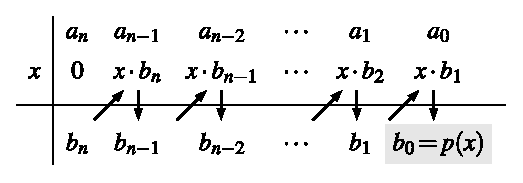
\includegraphics[width=0.45\linewidth]{Kap3_1}
			\end{figure}
		\item \textbf{Wie sind die Lagrange-Polynome definiert? Welche Eigenschaften haben sie?}
			\begin{align*}
				\ell_i(x)&=\frac{(x-x_0)(x-x_1)\cdots\reallywidehat{(x-x_i)}\cdots(x-x_n)}{(x_i-x_0)(x_i-x_1)\cdots\reallywidehat{(x_i-x_i)}\cdots(x_i-x_n)} \\
				\ell_i(x_j)&=\delta_{ij} =
					\begin{cases}
						1, & \text{falls } i=j,\\
						0, & \text{falls } i\neq j.
					\end{cases} \nonumber
			\end{align*}
			Wobei die überdachten Terme wegzulassen sind.
		\item \textbf{Wie wird mit Hilfe der Lagrange-Polynome das Langrangesche Interpolationspolynom berechnet?}
			\begin{align*}
				p(x)=\sum_{i=0}^{n}y_i\,\ell_i(x), \quad p(x_j)=y_j
			\end{align*}
		
		\item \textbf{Erklären Sie die Begriffe Datenfehler, Verstärkungsfaktor, Lebesgue-Funktion und Lebesgue-Konstante in Zusammenhang mit der Polynominterpolation. Was ist die Kondition der Polynominterpolation?} \\
			An einer Stützstelle \(x_j\) kann ein Datenfehler \(\varepsilon_j\) auftreten.
			Führt man diesen in ein Lagrange-Polynom ein erhält man
			\begin{align*}
				\overline{p}(x)=\sum_{i=0}^{j-1}\left( y_i\,\ell_i(x)\right) + (y_j+\varepsilon_j)+\sum_{i=j+1}^{n}\left( y_i\,\ell_i(x)\right).
			\end{align*}
			Der Fehler \(\varepsilon_i\) wird also um den Faktor \(|\ell_i|\) verstärkt.
			Wenn alle Knoten mit Fehlern verseht sind ergibt sich
			\begin{align*}
				\overline{p}(x)=p(x)+\sum_{i=0}^{n}\left( \varepsilon_i\,\ell_i \right) .
			\end{align*}
			Falls die einzelnen Fehler durch \(\varepsilon_i\le\text{M}\) beschränkt sind erhält man für den absoluten Fehler die Abschätzung
			\begin{align*}
				\underbrace{|\overline{p}(x)-p(x)|}_\text{abs. Fehler Output}\leq \text{M}\underbrace{\sum_{i=0}^{n}\overbrace{|\ell_i(x)|}^{\kappa_{\text{abs},i}(x)}}_{\kappa_\text{abs}(x)}
				= \text{M}\cdot\kappa_\text{abs}(x).
			\end{align*}
			Wobei \(\kappa_{\text{abs},i}=|\ell_i(x)|\) der Verstärkungsfaktor für den Datenfehler in der Stützstelle \(i\) und die Lebesgue-Funktion \(\kappa_\text{abs}=\lambda_n(x)=\sum_{i=0}^{n}|\ell_i(x)|\) die absolute Kondition für die Polynominterpolation ist. Die schlechteste Konditionszahl \(\lambda_n(x)\) im Intervall \([\text{min}_ix_i,\text{max}_ix_i]\) nennen wir Lebesgue-Konstante und erhalten sie durch
			\begin{align*}
				\underset{x\in[\text{min}_ix_i,\text{max}_ix_i]}{\text{max}} \lambda_n(x):=\Lambda_n.
			\end{align*}
		\item \textbf{Was besagt der Satz über den Fehler des Interpolationspolynoms? Wie ist der Verfahrensfehler definiert?} \\
		
		\item \textbf{Wie sind die Tschebyscheff-Polynome definiert? Welche Eigenschaften haben sie?} \\
		
		\item \textbf{Wie berechnet man die Knoten für die Tschebyscheff-Interpolationspolynome im Intervall [−1, 1] bzw. [a, b]? Welche Vorteile hat die Verwendung von Tschebyscheff-Knoten im Vergleich zu äquidistanten Stützstellen.} \\
		
		\item \textbf{Wie lässt sich das dividierte Differenzenschema und das Newtonsche Interpolationspolynom verallgemeinern, falls in den Stützstellen auch noch Ableitungen vorgegeben sind?} \\
		
		\item \textbf{Wie wird mit stückweise konstanten Funktionen interpoliert?} \\
		
		\item \textbf{Wie wird mit stetigen, stückweise linearen Funktionen interpoliert?} \\
		
		\item \textbf{Was sind Hutfunktionen und welche Eigenschaften haben sie?} \\
		
		\item \textbf{Was für Eigenschaften besitzen kubische Splines? Was für Typen von kubischen Splines gibt es?} \\
		
		\item \textbf{Wieso ist es besser durch viele Punkte einen kubischen Spline zu legen, statt ein Interpolationspolynom zu verwenden?} \\
		
		\item \textbf{Wie wird auf einem rechteckigen Gitter zweidimensional interpoliert?} \\
		
		\item \textbf{Wie wird die zweidimensionale, stetige, stückweise lineare Interpolierende auf einem rechteckigen Gitter bestimmt?} \\
		
	\end{enumerate}